\documentclass[sigconf]{acmart}


\usepackage{amsmath}
\usepackage{algorithm}
% \usepackage[section]{placeins}
\usepackage[noend]{algpseudocode}
\usepackage{hyperref}
\usepackage{endfloat}
\renewcommand{\efloatseparator}{\mbox{}} % no new page between figures

\usepackage{booktabs} % For formal tables

\settopmatter{printacmref=false} % Removes citation information below abstract
\renewcommand\footnotetextcopyrightpermission[1]{} % removes footnote with conference information in first column
\pagestyle{plain} % removes running headers



\begin{document}
\title{Continuous Motion Detection Using Convolutional Neural Network and Recurrent Neural Network}


\author{Ajinkya Khamkar}
\orcid{1234-5678-9012}
\affiliation{%
  \institution{Indiana University}
  \streetaddress{P.O. Box 1212}
  \city{Bloomington} 
  \state{Indiana} 
  \postcode{47408}
}
\email{adkhamka@iu.edu}

% The default list of authors is too long for headers}
\renewcommand{\shortauthors}{K. Ajinkya}


\begin{abstract}

Object detection is fundamental and important Computer Vision task. Continuous object detection is an extension of object detection for continuous motion scenes. Traditional methodologies include estimating object displacement in subsequent scenes using optical flow methodology. Optical flow can be computationally expensive to compute making it unattractive for online learning methodologies. Deep Neural Network learning techniques present an alternative approach for determining continuous motion without explicitly computing the optical flow between subsequent frames.
\end{abstract}

\keywords{I523,HID211, Continuous Motion Detection, Convolutional Neural Networks, Object Detection, Deep Neural Networks}


\maketitle

\section{Introduction}

Object detection is fundamental and important Computer Vision task. Continuous object detection is an extension of object detection for continuous motion scenes. In section \ref{applications}, we discuss the scope and applications driven by continuous motion detection. In section \ref{experimentaldata}, we present the data that we use for our experiments. 

In section \ref{traditional}, we discuss traditional techniques used for continuous motion detection. Traditionally, hand crafted features \cite{articlezhou} and optical flow \cite{LK} between subsequent frames was used to detect continuous motion detection. We discuss the major drawbacks of using traditional optical flow and hand crafted feature based methods. These drawbacks can be overcome using newer deep learning techniques. 

We begin section \ref{newer} by discussing about deep convolutional neural networks and their application for object detection. We introduce certain naive methods that can be used to achieve continuous object detection. In section \ref{RNN}, we introduce Recurrent Neural Networks and their application for continuous object detection. We discuss long-short-term-memory networks a form of recurrent neural network which is designed to retain scene memory over long periods of time. We discuss implementations which use long-short-term-memory networks along with deep convolutional neural networks to improve the performance of the naive methods. 

In section \ref{approach}, we present an end-to-end approach and algorithm which can be trained in a single shot fashion with the gradient generated by long-short-term-memory network to train the object detection network. 

In section \ref{arch}, we discuss the our training methodology and training resources used for our experiment. In section \ref{results}, we present the results we achieved for training the model in an end-to-end fashion. In section \ref{conclusion}, we conclude our discussion.

\section{Applications}\label{applications}

The applications and scope of motion detection and object tracking has risen exponentially over the last decade. In recent years, we have seen several concepts of automated vehicular driving, physical robots aiding human-centric activities, aerial drone technologies replacing traditional delivery schemes, virtual reality based systems tracking human movement habits and learning from those and use of motion tracking in popular sports for crucial decision making\cite{sports}. Continuous motion detection and robotic vision remain at the crux of all the above applications. Traditionally, motion detection has also been used for security monitoring \cite{6139506} and tracking suspicious activities. Researchers have traditionally used object tracking methodologies to study human movement patterns, track bird, mammal and aquatic migration patterns and draw conclusions from them. Thus it remains important to introduce computationally efficient and online learning methodologies which can used for real time object motion detection.

\section{Data} \label{experimentaldata}

One of the major difficulties in training architectures for continuous motion detection is lack of availability of labelled data. Videos are a sequence of image frames and speed of motion is determined using the rate at which these frames are presented to the naked human eye. Additionally motion changes in subsequent frames is minimal and can be approximated to zero or no-motion. Human experts are required to annotate images by drawing bounding boxes around objects of interests in image frames. Few second long videos can have thousands of frames depending upon the frame rate. Several online platforms including amazons mechanical turk are used by researchers to create labelled data. Participants are paid for labelling scenes and hand annotating object locations. This makes the annotation task expensive and tedious. 

For this experiment we use Visual Object Tracking challenge dataset \cite{6755885}. The dataset has 16 videos corresponding to different action sequences, each action has on an average 400 motion frames. Each frame is further labelled with the object of interest and bounding box annotations. Each frame presents a single object of interest. Each object is under varied illumination, colour and shape conditions. Additionally the images are noisy and blurry replicating low resolution tracking devices traditionally found in the wild.  


\section{Traditional Approaches} \label{traditional}

Traditional methods involve use of hand crafted features including hand annotating interest points on objects within images and then tracking the motion of interest points in subsequent frames. Another traditional approach uses the bag of words representation of images or uses the histogram of oriented gradients \cite{articlezhou} approach to locate objects of interest in the images. These approaches have multiple severe drawbacks which we discuss further. 

\begin{itemize}
\setlength\itemsep{1em}
\item These approaches fail to scale for larger dataset with different objects of varied size and shapes. They suffer further from scale and illumination variance in continuous frames.

\item Researchers are tasked with detecting feature points within images, thus making this mechanically tasking and expensive.
\end{itemize}

Another important and popular approach for tackling continuous motion problems involves the computation of optical flow. Optical flow \cite{LK} computes the relative motion between pixels in subsequent frames. Optical flow uses the following assumption, given motion of the pixels in subsequent frames is small or negligible, the changes in intensity or brightness in subsequent frames will be constant or near zero.

\begin{align} \label{eqn2}
{I(x,y,t) = I(x+\Delta x, y+\Delta y, t+\Delta t)}
\end{align}

In equation \ref{eqn2} $I$ represents the pixel wise intensity across frames. If the movement is small the right hand side of the above equation can be approximated using the first order Taylor series 

\begin{align} \label{eqn3}
{I(x+\Delta x, y+\Delta y, t+\Delta t) = I(x,y,t) + \frac{\delta I }{\delta x} \Delta x + \frac{\delta I }{\delta y} \Delta y + \frac{\delta I }{\delta t} \Delta t}
\end{align}

\begin{align} \label{eqn4}
{\frac{\delta I }{\delta x} \Delta x + \frac{\delta I }{\delta y} \Delta y + \frac{\delta I }{\delta t} \Delta t = 0}
\end{align}

\begin{align} \label{eqn5}
{\frac{\delta I }{\delta x} \frac{\Delta x}{\Delta t} + \frac{\delta I }{\delta y} \frac{\Delta y}{\Delta t} + \frac{\delta I }{\delta t} \frac{\Delta t}{\Delta t} = 0}
\end{align}

\begin{align} \label{eqn6}
{\frac{\delta I }{\delta x} \frac{\Delta x}{\Delta t} + \frac{\delta I }{\delta y} \frac{\Delta y}{\Delta t} + \frac{\delta I }{\delta t} = 0}
\end{align}

\begin{align} \label{eqn70}
{\frac{\delta I }{\delta x} V_x+ \frac{\delta I }{\delta y} V_y = - \frac{\delta I }{\delta t}}
\end{align}

Here $V_x and V_y$ represent the optical flow in directions $x,y$ and the partial derivative represent the derivative of the image at pixel x and y. The equation has 2 unknowns and requires additional constraints and equation to solve for the unknowns. Two popular approaches to estimate the optical flow include Lucas-Kanade method and Horn-Schunk method.  Lucas-Kanade \cite{LK} method solves for the unknown using the assumption, the motion for all pixels in a window centered around p between frames will be constant. Thus they solve for the equation.

\begin{equation} \label{eq7}
\begin{split}
I_x (p_1) V_x + I_y (p_1) V_y = - I_t (p_1) \\
I_x (p_2) V_x + I_y (p_2) V_y = - I_t (p_2) \\
\vdots
\end{split}
\end{equation}

Here $I_{x,y}(p_n)$ represents the partial derivative of the intensity at location $x,y$ and $V_{x,y}$ is the optical flow at pixels within the window centered around p. 

Horn-Schunk \cite{Horn:1980:DOF:888857} method assumes the flow of pixels across the image in subsequent frames is smooth and distortion free. It approximates the optical flow by solving the equations 

\begin{equation} \label{eq8}
\begin{split}
I_x(I_x u + I_y v + I_t) - \alpha^2 \Delta u = 0 \\
I_y(I_x u + I_y v + I_t) - \alpha^2 \Delta v = 0 \\
\end{split}
\end{equation}

where $\Delta = \frac{\delta^2}{{\delta x}^2} + \frac{\delta^2}{{\delta y}^2}$ is the Laplacian operator. The above approaches suffer from multiple drawbacks which we discuss below. 

\begin{itemize}
\setlength\itemsep{1em}
\item These approaches require calculation or approximation of the higher order polynomials making it computationally inefficient for scaling.

\item These approaches are make several assumptions about the images. These assumptions fail to hold in the wild.

\item These approaches heavily depend on the constant brightness principle and fail to perform well for images with varying brightness, illumination, distortion and color.

\end{itemize}

\section{Newer Approaches} \label{newer}

\subsection{Convolutional Neural Networks}

Recent research on continuous motion detection is heavily focused on the use of deep convolutional neural networks for the task object detection. Deep convolutional neural networks \cite{NIPS20124824} are characterized by the movement of the convolution operator over the input image. Each convolution operatorion is called a filter and the filter is responsible for capturing unique patterns appearing within the input image. Filters use non-linear activation helping the network capture non linear relationships that may exist within the input data. One complete traversal of a filter over the input results in a feature representation. Multiple such representations are stacked at every convolution layer to create feature maps. Feature maps capture the various patterns that occur across images. Further, these feature maps extract patterns at different scales and intensities making the model robust to affine transformations and scale invariance. These feature maps are further mapped to an embedding layer which extracts important features that appear across these feature maps. This embedding is further fed to a fully connected network which is responsible for making output decisions. Similar images or images belonging to the same class have repetitive patterns. These repetitive patterns are captured within the low representation embedding of the image. Thus, neural networks are invariant to scale, illumination and affine transformation.

\subsection{Object Detection}

Object detection is the task of identifying various objects that are present within the image scene. Feature maps capture various object level information at different scales. The approach to object detection is simple. Along with the classification output the network outputs multiple regression outputs, the regression outputs signify the approximated location of an object in a scene. During backpropagation, neurons which generated the feature map for the object are penalized using mean squared error for misidentifying the location of the object. With a large dataset and over multiple iterations, the network learns to identify feature maps corresponding to objects within the scene. As the network is invariant to scale and affine transformations it generalizes well for similar objects with different sizes, shapes and colours under different illumination and environmental constraints.


Multi-object detection is task of identifying multiple objects within the scene. The task is complex as compared to single object detection problem. Traditional approaches involved using a sliding window of fixed dimension across feature maps and feeding each window to the fully-connected network. The network decides whether the window contains an object. This approach has the following drawbacks

\begin{itemize}
\setlength\itemsep{1em}
\item As the window slides per pixel, large number of input vectors are generated and fed to the fully connected network making it computationally inefficient

\item Since the size of the window is fixed, it fails to capture objects of varying scale

\item Overlapping of windows leads generates large number of false positives.

\end{itemize}

Girshick et al. \cite{DBLP:journals/corr/GirshickDDM13}, use external image processing techniques such as histogram of oriented gradients and pixel wise unsupervised segmentation to generate candidate object boxes, thereby reducing the number of possible input vectors. Ren et al. \cite{DBLP:journals/corr/RenHG015}, use the existing annotations available within the dataset to generate the candidate boxes and generate equal random boxes from different part of the image to generate negative examples, classified as background. Redmon et al. \cite{DBLP:journals/corr/RedmonDGF15}, propose a single sweep over the input image and train the network for multiple object detection in an end-to-end fashion. 

\subsection{Recurrent Neural Networks} \label{RNN}

Recurrent neural networks \cite{DBLP:journals/corr/Lipton15} are a variant of traditional neural networks. They are characterized by a recursive loop which feeds the output of the network back as an input to the network. This allows information to persist within the network. Recurrent neural networks have successfully been used for addressing multiple challenges. They are extensively used for natural language modelling, speech recognition, cognitive science and time-series analysis. This is due to their excellent ability to model and memorize sequences for long temporal duration. Vanilla recurrent neural network has two major drawbacks. We discuss them below.

\begin{itemize}
\setlength\itemsep{1em}
\item Recurrent neural networks can have several input units depending upon the temporal duration of the activity. When the input signal flows from one unit within the network to the next, it is attenuated using non-linear activation. After flowing through several units within the network, the input signal dies off. This problem is traditionally known as the gradient vanishing problem. If the gradient vanishes during the forward pass of the network, the ability of the network to learn via gradient descent through backpropagation is weakened. Thus, the network fails to learn sequences over longer duration.

\item Recurrent neural networks also suffer from gradient explosion problems. An unrolled version of a recurrent neural network is equivalent to feed forward neural networks. During backpropagation the gradient generated by the final layer is accumulated over the layers, leading to drastic unstable changes in the weights of the networks.

\item Vanilla recurrent neural networks also suffer due to lack of inbuilt correction mechanism. Advanced versions of Recurrent neural networks can correct the weights of the recursive loop to control the influence of previous inputs on the correct input thereby preventing the weights from exploding.

\end{itemize}

\subsection{Long Short Term Memory Network}

Long short term memory network \cite{Hochreiter:1997:LSM:1246443.1246450} is an advanced variation of the vanilla recurrent neural network. They overcome the gradient explosion and gradient vanishing drawbacks of the traditional recurrent network. They are characterized by a memory cell which holds sequential information. This characteristic of the network is important in tracking motion of objects in subsequent frames of video. The memory cell is connected to 4 gates which determine the flow of information to and from the memory cell and within the network.

\begin{itemize}
\setlength\itemsep{1em}
\item Forget gate: Forget gate determines the influence previous outputs have on the current unit of the long short term memory network. The decision of the gate is driven by the rest of the network. This is essential, as blocking the flow of information to the memory cell reduces the compounding error, stabilizing the training and preventing the gradients to explode during backpropagation

\item Input gate: Input gate determines, the joint influence of the current input and the output of the previous layer has on the unit of the long short term memory network. The decision of the gate is driven by rest of the network. Input gate along with the forget gate determine the sequence the network is tasked to remember.  

\item Output gate: Output gate determines the influence the current unit has on future units. 

\end{itemize}

\subsection{Working}

The network first determines the importance of the previous output with respect to the state of the current unit. The units within the forget gate $f_t$ are driven to either 1 or 0 by the rest of the network.

\begin{align} \label{eqn15}
f_t = \sigma (W_f [h_{t-1},x_t])
\end{align}

The network then determines the influence of the input to the current unit of the long short term memory network. The weights of the input gate $I_t$ unit is driven to either 1 or 0 by the rest of the network. 

\begin{align} \label{eqn16}
i_t = \sigma (W_i [h_{t-1},x_t])
\end{align}

\begin{align} \label{eqn17}
\hat{C_t} = tanh (W_c [h_{t-1},x_t])
\end{align}

$ \hat{C_t} $ determines the intermediate update vector of the unit 

The memory cell of the current unit is then updated with thew new update vector determined by the following equation

\begin{align} \label{eqn18}
C_t = f_t * C_{t-1} + i_t * \hat{C_t}
\end{align}

The network outputs the following to drive the future units


\begin{align} \label{eqn19}
o_t = \sigma (W_o [h_{t-1},x_t])
\end{align}

\begin{align} \label{eqn20}
h_t = o_t * tanh(C_t)
\end{align}


\section{Approach} \label{approach}

We present an end-to-end approach for continuous motion detection and object tracking using deep convolutional neural network and long short term memory networks. As the approach is end-to-end, we can train all networks in a single shot and optimize neural network layer weights using a single loss metric and gradients. 

\begin{algorithm}

\caption{Single Shot motion tracking}\label{SSDLSTM}

\begin{algorithmic}[1] 
\State{Load video frames $f_i$, ground truth labels $l_i$, bounding box annotations $b_{i,j}$}
\State {Pre-process $f_i, l_i, b_{i,j}$  }
\Procedure{Model}{$f_i,l_i,b_i$}
\State{Create arbitrary input batch of 64 frames, labels, annotations}
\State{Feed batch to $CNN$ }
\State{Generate embedding $E_{CNN}$, annotations $b_{CNN}$, label $l_{CNN}$}
\State{Concatenate $E_{CNN}$, $b_{CNN}$, $l_{CNN}$} to form long vector $V_{CNN}$
\State{Feed $V_{CNN}$ to LSTM}
\State{Predict approximated location of object in future frame $b_{+1}$}
\State{Compute joint loss and and gradients $g$ and update network weights}
\EndProcedure
\State{Save Model}
\end{algorithmic}

\end{algorithm}

Our approach is pretty similar to the one presented by Valipour et al. \cite{ DBLP:journals/corr/ValipourSJR16} which was used for end-to-end video segmentation. The approach is simple, we begin by feeding a video frame from an arbitrary position within the video through a deep convolutional network.  We concatenate lower dimensional embedding of the input frame along with the class of the object and its location to form a one dimensional long vector. This vector is then fed to a stacked long short term memory architecture. The output of the long short term memory network is approximated location of the object in the subsequent frame. 

\begin{figure}  [htbp]
  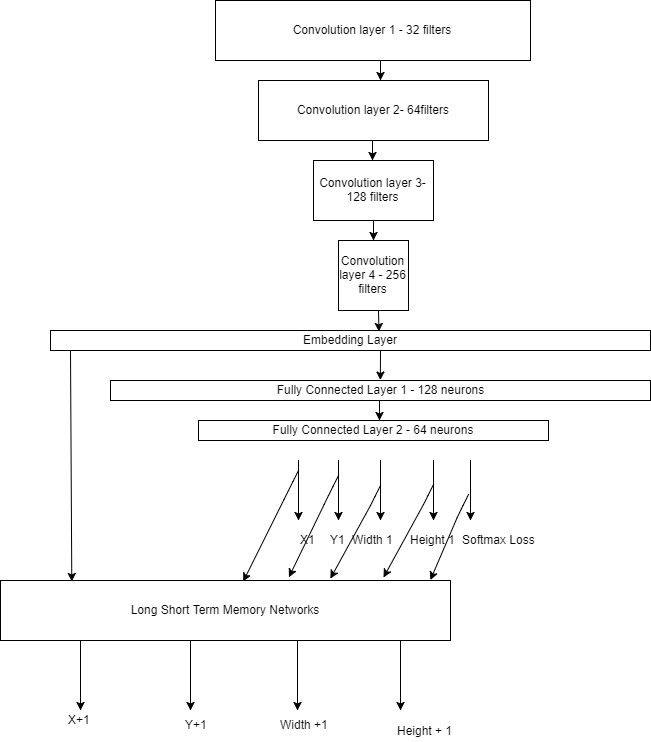
\includegraphics[width=\linewidth]{images/model.png}
  \caption{Model Architecture}
  \label{Model architecture}
\end{figure}

We pre-train the deep convolutional neural network for the dataset \cite{DBLP:journals/corr/YosinskiCB}. Pre-training the neural network helps it to converge faster and stabilizes the training of the long short term memory networks which we introduce further. We believe a pre-trained deep neural network architecture trained on the ImageNet dataset will further improve the performance and generalizability of the model for unseen data samples. We do not present results or analysis for ImageNet trained architectures in this experiment. We use the deep convolutional network to extract a lower level embedding of the input image. Lower level embedding captures features present within an image. 

We believe, the class of the object plays an important role in determining the rate of change in motion of the objects in subsequent frames {e.g. Divers leaning forward, motion change of a car as compared to bicycles will be higher}. Additionally, we use the current location of the object as a correction mechanism for the long short term memory network to prevent it from diverging from the actual motion the object in subsequent frames. We use a time stamp of 5 frames to determine the location of the object in the $6^{th}$ frame. We believe 5 frames captures the relative motion of the object between frames. We jointly try to minimize a multiple loss function.

\subsubsection{Cross-entropy loss}

\begin{align} \label{eqn9}
{\mathcal{L} = -\frac{1}{n} \sum_{i=1}^n y^{(i)} \ln \delta(x^{(i)}) + \left(1 - y^{(i)}\right) \ln \left(1 - \delta(x^{(i)})\right)}
\end{align}

$x_i$ is the input samples and $y_i$ is the output for the corresponding input samples. $\delta(x_i)$ is the output of the activation function

\begin{align} \label{eqn10}
{\delta(x) = \frac{1}{1 + e^{-Wx-b}}}
\end{align}

$W$ and $b$ represent the weights and bias of the neural network. We minimize the cross-entropy loss for the classification task.

\subsubsection{Mean-square loss}

\begin{align} \label{eqn11}
{MSE={\frac  {1}{n}}\sum _{{i=1}}^{n}({\hat{Y_{i}}}-\delta(x^{(i)})^{2}}
\end{align}

$x_i$ is the input samples and $y_i$ is the output for the corresponding input samples. $\delta(x_i)$ is the output of the activation function

\begin{align} \label{eqn1000}
{\delta(x) = \frac{1}{1 + e^{-Wx-b}}}
\end{align}

$W$ and $b$ represent the weights and bias of the neural network. We minimize the mean square error loss for the regression task.

We minimize the cross-entropy and mean squared loss generated by the deep convolutional network in predicting and localizing the object in the video frame. In an end-to-end fashion, we allow the loss generated by the long short term memory network to flow through the convolutional neural network to jointly minimize the loss in predicting the location of the object in the next frames. 

\subsection{Salient Features of Architecture} \label{arch}

\begin{itemize}
\setlength\itemsep{1em}

\item The input size of frames vary for different videos. Frame heights are centered on 240 pixels and width on 360 pixels. We use a fixed dimension of 120 x 120 pixels for this experiment. The number of frames per video is high, to prevent computational bottlenecks we use a lightweight convolutional neural network architecture. Another benefit of a light weight architecture is it allows the network to be deployed on low powered devices. 

\item We use 5 convolutional layers with 32, 64, 128 and 256 filters respectively. Each filter is of the size 3 x 3. We use the Adam optimizer for our experiments.

\item with each convolutional pass, we reduce the dimensions of the image by half thereby further improving the computational efficiency of our model. We use strides instead of the traditional pooling architecture. Pooling leads to loss of visual information and deteriorates object localization performance. 

\item We use Rectified linear units for activation in each of our layers. Rectified units prevent gradient saturation and are computationally efficient to calculate.

\item  Additionally, as we are dealing with a medium sized dataset, our model is prone to over fitting. To prevent over fitting, we couple every convolutional neural network layer with a dropout layer. Dropout serves as a regularizer for neural network architectures as it randomly drops out multiple neurons in the every hidden layer, leading to high misclassification and mean square error and penalizing the neurons forcing them to generalize for all classes.

\item We use affixed batch size of 64 temporal frames for our experiment. We randomly select the starting frame so as to prevent our network from over fitting on the sequence of the video frames.

\item We use a 2 layered stacked long short term memory network with 16 and 4 units each. We use hyperbolic tangent as an activation for the recurrent neural network. We use categorical cross-entropy loss for the classification task and we use mean squared error for the regression task 


\end{itemize}

\subsection{Training}

We train our model on Indiana University's cluster computing resource Big Red 2 and Karst. We use a total of 6 CPU's to pre-train our model for the classification and regression task and we use one graphical processing unit along with 6 CPU's and 96 cores to train our end-to-end model.  We train our model for 100 iterations. For each iteration during pre-training we randomly sample a batch of 64 images, labels and bounding boxes for the classification and regression task. As we are dealing with a medium sized dataset, the error converges quickly. It takes 6 hours to pre-train our model on the above stated configuration. For end-to-end training we use the following approach. We train the model for 75 iterations. In Each iteration, we sample a sequence of 128 video frames randomly and pass it to our model to generate future location of our object in context. We repeat this procedure for 100 randomly sampled sequences of 128 video frames. Random sampling improves the generalizability of our approach. Additionally as we sample randomly, we are required to repeat this approach multiple times to ensure our model trains on all action sequence. Training the model in an end-to-end fashion requires 12 hours on CPU configuration and takes about 3 hours with the Graphical Processing Unit. 


\section{Evaluation} \label{results}

We evaluate multiple metrics during training. We try and minimize the cross-entropy loss for the classification task, and minimize the mean-squared error loss for the object position in current frame and future frame. We achieve a cross-entropy loss of 2 \% in relative context. Additionally, each iteration uses a randomly sampled sequence of video frame thus indicating our model generalizes well for different actions being performed in the video. The mean squared error loss for the future frame decreases with every iteration indicating our model is able to learn motion sequence in continuous frame. The loss decreases to a minimum of 5 \% in relative context which is significant as the loss is jointly computed for all 4 coordinates of the future frame simultaneously. Figure 1, shows the training loss compared to validation loss. We can clearly infer that the model performs well on the validation set, at times exceeding the training accuracy.

 
\begin{figure}[htbp]
  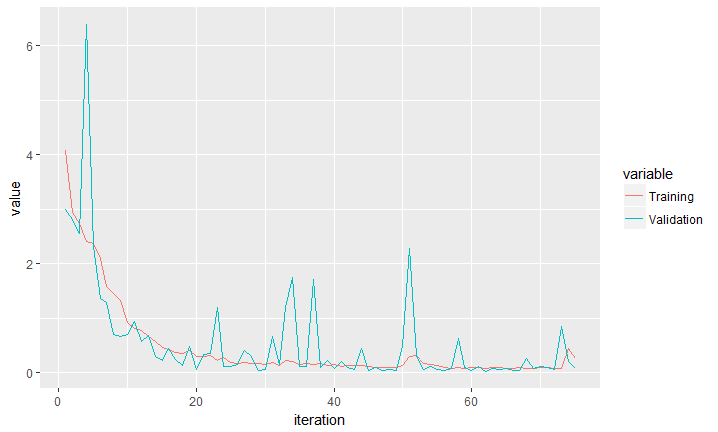
\includegraphics[width=\linewidth]{images/Plot.png}
  \caption{Train versus validation loss function}
  \label{fig:Evaluation plot}
\end{figure}


\begin{figure}[htbp]
  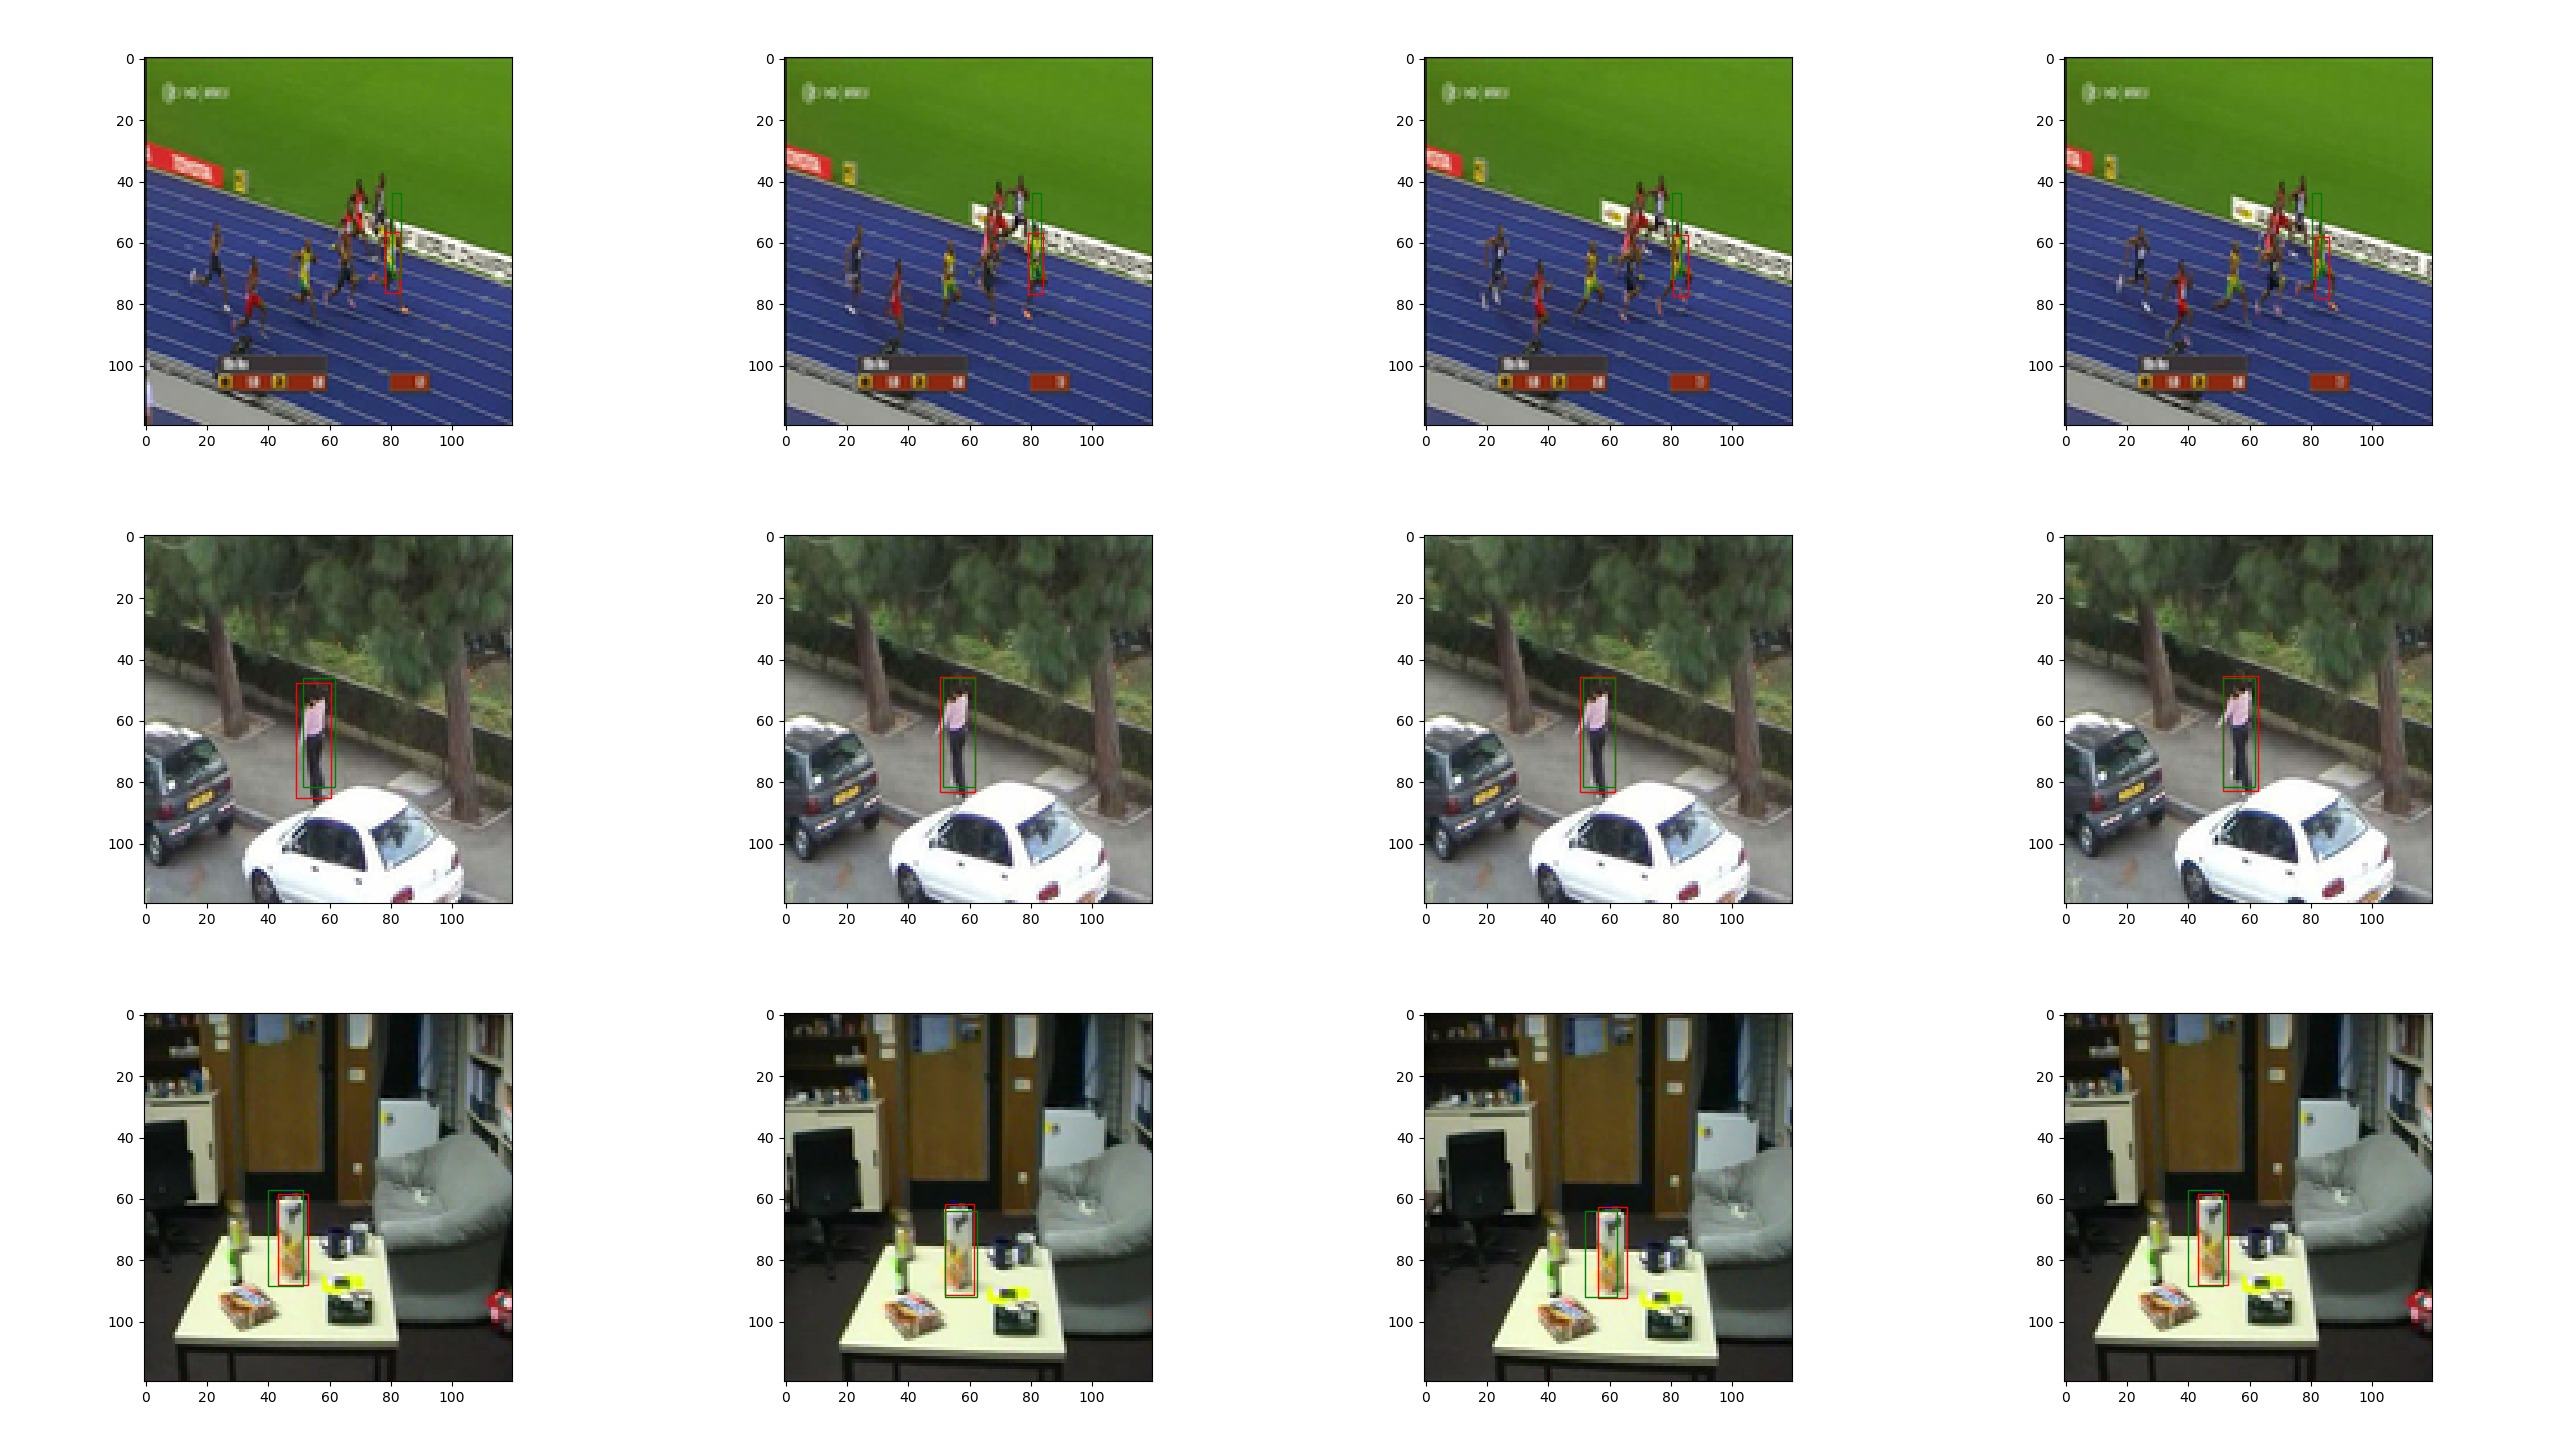
\includegraphics[width=\linewidth]{images/Predicted.jpg}
  \caption{Predicted Examples, green indicates predicted value, red indicates actual location}
  \label{fig:Prediction Examples}
\end{figure}


\begin{table}[]
\centering
\caption{Loss Table-Training}
\label{table1}
\begin{tabular}{llll}
Iteration & Training Joint Loss & Training LSTM Loss & Training Cross Entropy Loss \\
1         & 2.9984              & 0.0174             & 2.7480                      \\
10        & 0.7004              & 0.0069             & 0.6378                      \\
20        & 0.0588              & 0.0035             & 0.0175                      \\
30        & 0.0470              & 0.0067             & 0.0014                      \\
40        & 0.0862              & 0.0044             & 0.0372                      \\
50        & 0.4786              & 0.0120             & 0.4142                      \\
60        & 0.0349              & 0.0041             & 2.3931e-04                  \\
70        & 0.0726              & 0.0038             & 0.0141                     
\end{tabular}
\end{table}

\begin{table}[]
\centering
\caption{Loss Table- Validation}
\label{table2}
\begin{tabular}{llll}
Iteration & Validation Joint Los & Validation LSTM loss & Validation Cross entropy Loss \\
1         & 4.0735               & 0.0296               & 2.8767                        \\
10        & 0.9193               & 0.0071               & 0.8033                        \\
20        & 0.2893               & 0.0044               & 0.2122                        \\
30        & 0.1720               & 0.0035               & 0.1120                        \\
40        & 0.1459               & 0.0041               & 0.0836                        \\
50        & 0.1347               & 0.0040               & 0.0678                        \\
60        & 0.1028               & 0.0034               & 0.0510                        \\
70        & 0.0745               & 0.0028               & 0.0306                       
\end{tabular}
\end{table}


\section{Conclusion} \label{conclusion}

Object and motion tracking is a difficult task. We presented traditional approaches to motion tracking and their computational flaws. We further presented a low powered light weight approach to tackle object and motion tracking using convolutional neural networks and recurrent neural networks. Our model fails to generalize for certain video sequences and tracks well for others. This we believe is due to reduced training time and and small sized dataset. Use of heavier architecture introduces computation bottlenecks and places high emphasis on object detection. By using recurrent neural networks we compensate for object localization mistakes made by our lightweight convolutional neural network by studying the apparent motion of the object in frames. We present competitive results on difficult benchmark dataset. We emphasize pre trained deeper networks on ImageNet dataset can improve the performance and generalizability of our approach but it loses the essence of the light weight architecture. We propose further improvements can be achieved by combining the best of both worlds. A two stream convolutional neural network with video frames and low resolution computationally efficient optical flow can improve the performance of our approach. 


\bibliographystyle{ACM-Reference-Format}
\bibliography{report} 

\end{document}


